\documentclass[11pt]{article}
\usepackage[margin=1.0in]{geometry}
\usepackage{setspace}
\usepackage{amsmath}
\usepackage{pdflscape}
\usepackage{fancyhdr}
\usepackage{listings}
\usepackage{tikz-qtree,tikz-qtree-compat}

\usepackage{tikz}
\pagestyle{fancy}
\lhead{CS 4610 Written Assignment 2}
\rhead{Zihao Wang (zw2rf)}
\cfoot{\thepage}
\renewcommand{\headrulewidth}{0.4pt}
\renewcommand{\footrulewidth}{0.4pt}
\renewcommand{\thesubsection}{\alph{subsection}.}
\begin{document}
\thispagestyle{empty}
\title{CS 4610 Written Assignment 2}
\author{Zihao Wang (zw2rf)}
\date{\today}
\maketitle
\doublespacing
\section{Write a context-free grammar for the language $L_{3} = L_{1} \cap L_{2}$}
$$S \rightarrow aTa \mid a$$
$$T \rightarrow XTX \mid \epsilon \mid a \mid b$$
$$X \rightarrow a \mid b$$

\textbf{Optional question:} I believe the intersection of a context-free language and a regular language is always context-free as regular language is a subset of context free language.

\section{Consider the grammar}
$$S \rightarrow aSb$$
$$S \rightarrow Sb$$
$$S \rightarrow \epsilon$$
\subsection{Give a one-sentence description of the language generated by this grammar.}
This grammar accepts strings starting with $m$ a's followed by $n$ b's where $0 \le m \le n$.  

\subsection{Show that this grammar is ambiguous by giving a single string that can be parsed in two different ways. Draw both parse trees.}
The string abb could be parsed into two different trees: \\
\begin{center}
\Tree [.S a [.S [.S $\epsilon$ ] b ] b ].S
\hskip 1in
\Tree [.S [.S a [.S $\epsilon$ ] b ] b ].S
\end{center}
\subsection{Give an unambiguous grammar that accepts the same language as the grammar above.}
$$S \rightarrow aRbT \mid \epsilon$$
$$R \rightarrow aRb \mid \epsilon$$
$$T \rightarrow bT \mid \epsilon$$

\section{Draw a parse tree for the expression.}
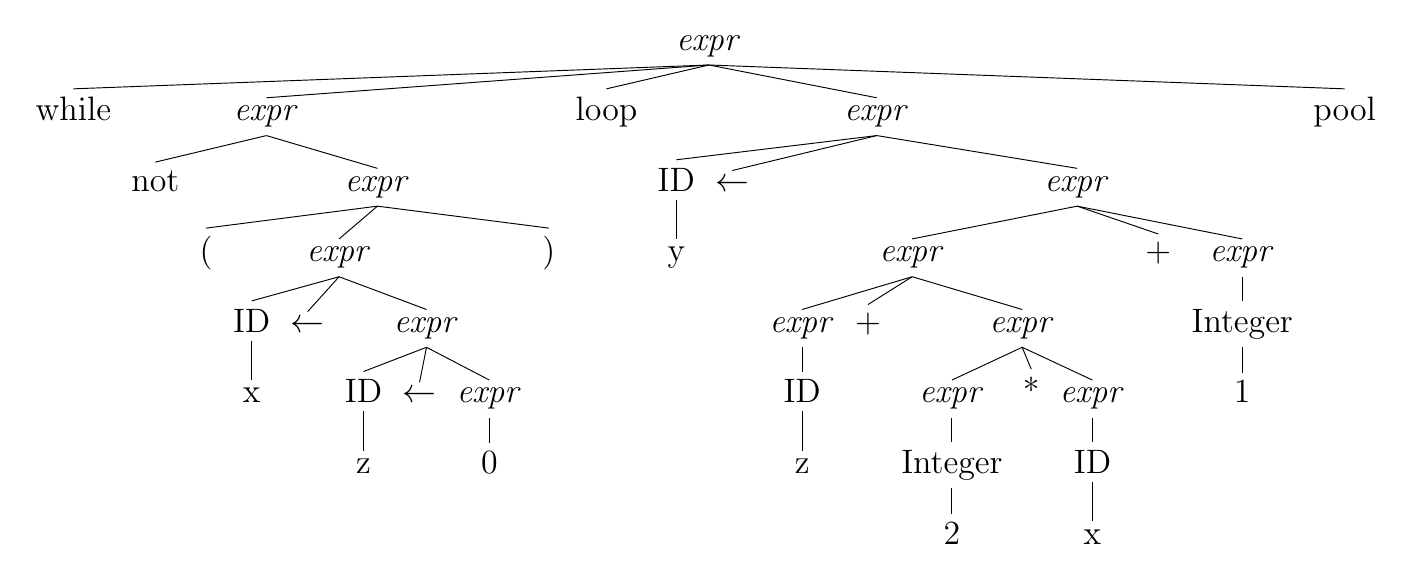
\begin{tikzpicture}[scale=.85, every tree node/.style={font=\Large,anchor=base}]
\Tree [.\textit{expr} while 
                 [.\textit{expr} not 
                        [.\textit{expr}
                        ( 
                        [.\textit{expr}
                        [.ID x ] $\leftarrow$  [.\textit{expr} [.ID z ] $\leftarrow$ [.\textit{expr} 0 ] ] ] ) ] ].\textit{expr}
                 loop 
                 [.\textit{expr} [.ID y ] 
                        $\leftarrow$ 
                        [.\textit{expr} [.\textit{expr} [.\textit{expr} [.ID  z ] ] 
                                      + 
                                      [.\textit{expr} [.\textit{expr} [.Integer 2 ] ] 
                                             * 
                                             [.\textit{expr} [.ID x ] ] ] ] + [.\textit{expr} [.Integer 1 ] ] ] ] 
                 pool ].\textit{expr} 
\end{tikzpicture}


\section{Give an example of a grammar that is $LL(3)$ but not $LL(2)$}
$$S \rightarrow abcS \mid abaS \mid abb$$



\end{document}